\section{Реализация} \label{sub24}

\subsection{Структура модуля} \label{sub241}

Модуль подсветки синтаксиса GRIP~DSL реализован на~языке GDSL(Groovy~DSL) диалекте, который предназначен для подсветки синтаксиса языков DSL, написанных на~Groovy, в~интегрированной среде разработки IntelliJ~IDEA.

Модуль состоит из~двух частей:

\begin{itemize}
	\item{функция определения контекста работы модуля;}
	\item{функция разбора файла и~определения грамматических конструкций, которые необходимо подсветить.}
\end{itemize} 

Определение контекста происходит посредством вызова специальной функции \texttt{context} с~передачей параметров, которые определяют место, где должны подсвечиваться грамматические конструкции языка GRIP~DSL, это может быть:
\begin{itemize}
	\item{расширение файла;}
	\item{полное имя файла;}
	\item{грамматическая конструкция (блок кода, тело метода и т.д.).}
\end{itemize} 

В реализованном модуле контекст определяется как любое замыкание \footnote{Замыкание~--- блок кода (или анонимная функция), который при выполнении имеет доступ к~переменным того контекста, в~котором он был объявлен. С~другой стороны, замыкание являются объектом, который может быть передан в~другие методы, сохранен в~переменных, и~т.п.}.

Разбор файла и~выделение новых полей и~их~типов реализованно в~функции \texttt{contributor}, которая на~вход принимает контекст исполнения (имя файла, место вызова), а~на~выходе неявно возвращает список новых полей и~их~типов, которые необходимо подсветить.

\newpage

\subsection{Интеграция модуля с IDE} \label{sub242}

Процесс взаимодействия IDE с~модулем GDSL представлен на~рис.~\ref{img:seq}.

\begin{figure}[ht]
	\centering
	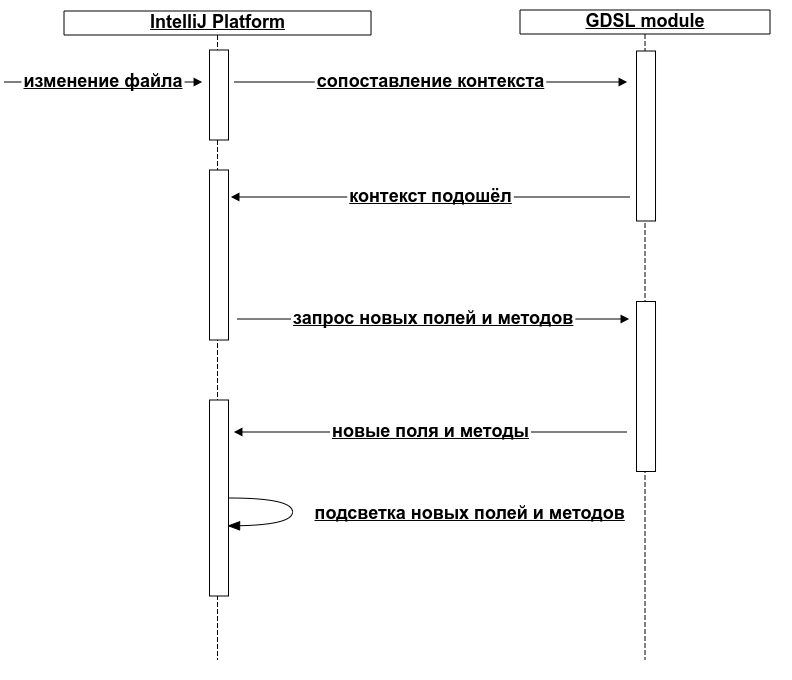
\includegraphics [scale=0.6] {seq}
	\caption{Взаимодействие IDE с~модулем GDSL}
	\label{img:seq}
\end{figure}

При каждом действии пользователя (нажатие на~клавишу) IntelliJ~IDEA обращается к~GDSL-модулю, который находится в~проекте, и~передаёт ему контекст. GDSL-модуль сопоставляет переданный контекст исполнения со~своим. Если контекст совпадает, то~модуль вызывает функцию \texttt{contributor}, в~которой происходит разбор файла и~поиск новых грамматических конструкций (динамических полей), определенных в~GRIP DSL. Результатом работы модуля является набор имен и~типов полей, которые соответствуют синтаксису GRIP DSL. Среда IntelliJ~IDEA подсвечивает эти поля и~делает проверку типов.